\chapter{Einfache Quantensysteme\label{chapter:einfache-quantensysteme}}
\lhead{Einfache Quantensysteme}
\rhead{}
In diesem Kapitel beschreiben wir einige einfache Quantensysteme und
entwickeln einen daf"ur geeigneten mathematischen Aparat. Dieser
Apparat ist bereits ausreichend, um zu erkl"aren, wie ein Quantencomputer
funktionieren k"onnte.

\section{Quantenmechanik als Zustandsmechanik}
\rhead{Quantenmechanik als Zustandsmechanik}
Eine Herleitung der Quantenmechanik im Stile des Beweises eines mathematischen
Satzes ist nat"urlich nicht m"oglich, und soll auch nicht versucht werden.
Hingegen sollen die wichtigsten Prinzipien aus einer heuristischen
Diskussion ``erraten'' werden. 

\subsection{Begriff des Zustandes}
In der Quantenmechanik gibt es kaum Experimente mit einzelnen Objekten.
Atome, Elektronen und Photonen sind einfach zu klein, oder gar nicht
isoliert herzustellen\footnote{Wir wissen, dass Protonen und Neutronen aus
Quarks zusammengesetzt sind, aber es ist nicht m"oglich, einzelne Quarks
zu isolieren (Confinement).}.
Vielmehr werden solche Experimente immer
an einer grossen Zahl von gleichartigen Objekten.
Sinnvolle Vorhersagen "uber den Ausgang eines solchen Experiments
sind allerdings nur m"oglich, wenn alle
Teilchen in allen f"ur das Experiment wesentlichen Aspekten
nicht unterscheidbar sind. Man kann dann sagen, dass sich die
Teilchen alle im gleichen {\em Zustand} befinden, wenn sie in
das Experiment eintreten.
\index{Zustand}

Dieser abstrakte Zustandsbegriff ist eine Verallgemeinerung konkreter
Arten von Zust"anden, wovon wir ein paar Beispiele nennen wollen.

Atome setzen sich aus einem Kern aus Protonen und Neutronen und einer
H"ulle aus Elektronen zusammen.
Durch Absorbtion von Photonen k"onnen Eletronen in der H"ulle Energie
aufnehmen, ein solches angeregtes Atom befindet sich in einem anderen
Zustand als eines, dessen Elektronen so viel Energie wie m"oglich
abgegeben haben.
Letzteres nennt man den Grundzustand eines Atoms.
Ein Experiment k"onnte also damit beginnen,
dass man einen Strahl von Atomen eines bestimmten Elementes herstellt,
die sich alle im Grundzustand befinden, oder alle auf die gleiche Art
angeregt worden sind.

Ein Zustand ist also festgelegt durch eine Menge von Eigenschaften,
die sowohl stetige oder diskrete Zustandsvariablen sein k"onnen.
Es ist keine wesentliche Einschr"ankung anzunehmen, dass Zust"ande
Vektoren in einem geeigneten Vektorraum sind.
Jede mathematische Struktur kann n"amlich in einem Vektorraum eingebettet
werden. Dies ist ganz offensichtlich f"ur die Geometrie, wo die Verwendung
eines Koordinatensystems jedes geometrische Problem in ein Problem "uber
Vektoren in einem dreidimensionalen Vektorraum. Die Details "uber den
Vektorraum, aus dem die Zust"ande kommen sollen, werden sp"ater festgelegt
werden. Wir schreiben daher einen Zustand als Vektor
\[
|\text{Beschreibung des Zustandes}\rangle
\]
in einem zun"achst nicht spezifizierten Vektorraum.

\index{CERN}
\index{LHC}
Am CERN werden im LHC Protonen auf eine sehr hohe Geschwindigkeit 
beschleunigt und dann zur Kollision gebracht. Es treffen also
Protonen mit einem bestimmten Impuls $p$ auf Protonen mit entgegengesetztem
Impuls $-p$. Es kollidieren also Protonen im Zustand $|p\rangle$ und
$|-p\rangle$. Das Experiment besteht dann darin zu messen, welche Arten von
Teilchen in welchen Zust"anden erzeugt worden sind.
Die Quantenmechanik hat
die Aufgabe, die m"oglichen Zielzust"ande vorherzusagen.

\index{Flasche!magnetische}
Eine magntische Flasche ist ein speziell konstruiertes magnetisches Feld,
in welchem geladene Elementarteilchen eingeschlossen werden k"onnen.
Den Teilchen in einer magnetischen Flasche kann einen Zustands zuschreiben,
der durch die Position bestimmt ist.
Wir k"onnten den Zustand eines Teilchens mit Position $x$ als $|x\rangle$
schreiben.

Die Quantenmechanik ist also eine Mechanik von Zust"anden: sie beschreibt,
unter welchen Umst"anden ein Teilchen von einem Zustand in einen anderen
Zustand "ubergef"uhrt werden k"onnen. 

\subsection{Observable}
\index{Observable}
Es ist charakteristisch f"ur die Quantenmechanik, dass sie mit diskreten
Mengen von Parameter zu tun hat. Zum Beispiel kann sich das Elektron eines
Wasserstoffatoms auf einer grossen Zahl von verschiedenen Energieniveaus
befinden. Gehen wir f"ur den Moment davon aus, dass es $n$ solche Zust"ande
gibt, die wir $|a_i\rangle, 1\le i\le n,$ schreiben wollen,
Ein $a$-Analysator zerlegt Teilchen im Zustand $|\psi\rangle$ in 
Teilchen in den Zust"anden $a_1,a_2,\dots,a_n$. Wir geben dies
schematisch durch das Diagramm
\index{Analysator}
\begin{center}
\includegraphics{graphics/analysator-1.pdf}
\end{center}
wieder.
\begin{figure}
\centering
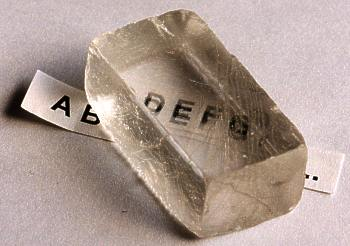
\includegraphics{images/calcit.jpg}
\caption{Kalkspat (Calcit) kann also Analysator f"ur die Polarisation
von Photonen dienen. Er zerlegt einen Strahl von Photonen in zwei
Strahlen mit orthogonaler Polarisierung.
\label{skript:calcit}}
\end{figure}
\index{Kalkspat}
\index{Calcit}
\index{Doppelbrechung}
Kalkspat (Calcit) (Abbildung~\ref{skript:calcit}) teilt einen Strahl
von Photonen auf in zwei Strahlen mit orthogonaler Polarisierung,
funktioniert also als Analysator f"ur zwei Polarisationsrichtungen
von Photonen.

\index{Analysatorkreis}
Man kann sich auch vorstellen, die vom Analysator getrennten Strahlen
wieder zusammenzuf"uhren, schematisch:
\begin{center}
\includegraphics{graphics/analysator-2.pdf}
\end{center}
Wir nennen ein solches Objekt einen {\em Analysatorkreis}, auch wenn wie
im n"achsten Beispiel nicht alle Pfade wieder zum Ausgang zusammengef"ugt
werden.

Wir k"onnen vor dem Zusammenf"ugen der Strahlen einzelne davon
blockieren, z.~B.~$a_2$:
\begin{center}
\includegraphics{graphics/analysator-3.pdf}
\end{center}
\index{Projektor}
Wir nennen diese Schaltung auch einen {\em Projektor}, er reduziert den
urspr"unglichen Strahl auf einen Zustand, dem die Komponenten $a_2$
fehlt. Nat"urlich k"onnen Projektoren f"ur eine beliebige Teilmenge
$A=\{a_{i_1},\dots, a_{i_k}\}$ definiert werden: der Projektor $P_A$
blokiert genau die Komponenten aus der Menge $A$.
\index{idempotent}
Damit die oben gezeigten Schemata f"ur Analysatoren ihre G"ultigkeit
haben, sollten Projektoren {\em idempotent}, d.~h.~zwei identische 
Projektoren wirken genau gleich wie ein einzelner, also $P^2=P$ oder
schematisch:
\begin{center}
\includegraphics{graphics/analysator-4.pdf}
\end{center}

Dies ist nur m"oglich, wenn die Wahscheinlichkeit, ein Teilchen nach
einem Projektor $P_{\{a_i\}}$ im Zustand $a_i$ zu finden, verschwindet.
Jeder andere Zustand muss hingegen unver"andert durchkommen, also
\[
P(a_i|a_j)=\delta_{ij}=\begin{cases}
1&\qquad i\ne j\\
0&\qquad\text{sonst.}
\end{cases}
\]
Ein solcher Satz von Zust"anden nennen wir eine Basis.

Nat"urlich sollen die Zust"ande alle m"oglichen Situationen abdecken
k"onnen, es sollte also keinen Zustand $|\psi\rangle$ geben, so dass
\[
P(a_i|\psi)=0\quad\forall i.
\]

\index{Observable}
In der Quantenmechanik sind also genau jene Gr"ossen messbar, f"ur die
es einen Analysator gibt, man nennt solche Gr"ossen {\em Observable}.
Die Polarisierung von Photonen, die Position oder der Impuls
eines Teilchens, das elektrische Dipolmoment eines Atoms sind alle
Observable.

\subsection{Photonenpolarisierung}
Betrachten wir als Beispiel Photonen und ihre Polarisation. 
Statt einer Basis aus den Zust"anden, die horizontal ($a_1$) und vertikal
($a_2$) polarisierte Photonen beschreiben, k"onnen wir auch zwei 
beliebige andere Polarisationsrichtungen $b_1$ und $b_2$ verwenden,
oder sogar rechts ($c_R$) und links ($c_L$) zirkul"ar polarisierte Photonen.
Seien also $b_1$ und $b_2$ gegen"uber $a_1$ und $a_2$ um den Winkel
$\alpha$ verdreht, dann wird die Intensit"at eines Strahls aus $a_2$
bei der Analyse mit $b_1$ und $b_2$ folgende Werte ergeben:
\begin{equation}
\begin{aligned}
P(b_1|a_2)&=\sin^2\alpha
&\qquad
P(b_2|a_2)&=\cos^2\alpha
\\
P(b_1|a_1)&=\cos^2\alpha
&
P(b_2|a_1)&=\sin^2\alpha.
\end{aligned}
\label{skript:polarisation-projektion}
\end{equation}
Die Wahrscheinlichkeiten sind proportional zu den Intensit"aten,
die proportional zum Quadrat der Amplituden sind (daher die Quadrate
in (\ref{skript:polarisation-projektion}).
\begin{figure}
\centering
\includegraphics{graphics/analysator-5.pdf}
\caption{Projektion des Zustandes $|a_2\rangle$ auf die beiden
um $\alpha$ verdrehten Basiszust"ande $|b_1\rangle$ und $|b_2\rangle$.
\label{skript:polarisation-rotation}}
\end{figure}
Man beachte, dass sich aus der Abbildung auch ableiten l"asst, dass
\begin{equation}
\begin{aligned}
P(a_1|b_1)&=\cos^2\alpha
&\qquad
P(a_1|b_2)&=\sin^2\alpha
\\
P(a_2|b_1)&=\sin^2\alpha
&
P(a_2|b_2)&=\cos^2\alpha.
\end{aligned}
\label{skript:polarisation-projektion-inverse}
\end{equation}
\index{Ubergangswahrscheinlichkeit@\"Ubergangswahrscheinlichkeit}
Man beachte, dass die "Ubergangswahrscheinlichkeiten
symmetrisch sind: $P(a_i|b_j)=P(b_j|a_i)$.
Ausserdem ergeben die Elemente $P(a_i|b_j), 1\le i\le n$ f"ur festes $j$,
zusammen den Wert $1$:
\[
\sum_{i=1}^nP(a_i|b_j)=1\quad\forall j.
\]
F"ur zirkul"ar polarisierte Photonen gilt immer 
\[
P(z_L|a_i)=P(z_R|a_i)=\frac12.
\]
Das Experiment in Abbildung~\ref{skript:linear-zirulaer} 
\begin{figure}
\centering
\includegraphics{graphics/analysator-6.pdf}
\caption{Experiment zur Messung des Zusammenhanges zwischen zirkul"arer
und linearer Polarisierung. Der rot hervorgehobene Block wird sp"ater
zur Berechnung von $P(c_L|a_2)$ verwendet.
\label{skript:linear-zirkulaer}}
\end{figure}
An der Stelle~1 ist der Strahl in Richtung $a_2$ linear polarisiert.
An der Stelle~2 ist er links-zirkul"ar polarisiert. Die Wahrscheinlichkeit,
das Intensit"atsverh"altnis der Strahlen zwischen den Punkten $1$ und $2$
ist
\begin{equation}
\frac{I_2}{I_1}=P(c_L|a_2)=\frac12.
\label{skript:intensitaetsverhaeltnis}
\end{equation}

\subsection{Doppelspaltexperiment}
\index{Doppelspaltexperiment}
\begin{figure}
\centering
\includegraphics{graphics/analysator-7.pdf}
\caption{Doppelspaltexperiment Teilchen mit gleichem Impuls oder Photonen
mit gleicher Wellenl"ange treffen von rechts auf eine Blende mit zwei
Spalten. Auf dem Schirm links werden die Teilchen gez"ahlt, die dort
eintreffen. Es entsteht ein Interferenzmuster.
\label{skript:doppelspalt-bild}}
\end{figure}
Das ber"uhmte Doppelspaltexperiment (Abbildung~\ref{skript:doppelspalt-bild})
erzeugt zun"achst einen Strahl
von Teilchen, die alle den gleichen Impuls $p$ haben, wir haben also
Teilchen im Zustand $|p\rangle$. Dieser Strahl
wird dann auf die zwei Spalte gerichtet. Dadurch wird der Strahl
beeinflusst, es entsteht also ein neuer Zustand, den zu berechnen
wir uns f"ur sp"ater zur Aufgabe machen wollen.
Im Moment bezeichnen wir diesen Zustand nach dem Doppelspalt 
als $|\psi\rangle$.

Gemessen wird dann, mit welcher Wahrscheinlichkeit
ein Teilchen im Zustand mit Position $y$ auf dem Schirm
gemessen wird, wenn das Teilchen im Zustands $|\psi\rangle$
ist. Dies ist ein bedingte Wahrscheinlichkeit, die wir also
$P(y|\psi)$ geschrieben werden kann.

Wir k"onnen dieses Experiment auch mit dem bisher entwickelten
Formalismus analysieren.
Zun"achst k"onnen wir die Blende als einen Analysator auffassen, der
den Strahl aufspaltet in verschiedene Zust"ande von Teilchen, die
den einen oder anderen Spalt traversiert haben.
Die Zust"ande $B_1$, $B_2$ und $B_3$ entsprechen Teilchen, die die
Blende nicht passiert haben. Die Zust"ande $S_1$ und $S_2$ entsprechen
Teilchen, die durch die beiden Spalte $S_1$ und $S_2$ geflogen sind.

Die unendlich vielen m"oglichen Positionen $y$ auf dem Schirm
k"onnen wir ebenfalls auf diskrete Zust"ande abbilden.
Dazu unterteilen wir den Schirm links in
disjunkte Zonen, die das Eintreffen eines Teilchens registrieren k"onnen.
Ein Teilchen kann offenbar nur in jeweils einer Zone registriert werden.
Bezeichnen wir die den Zustand eines Teilchens, welches in der Zone mit
der Nummer $i$ registriert wird, mit $y_i$, dann funkioniert der Schirm als
eine Kombination von Projektoren auf die Zust"ande $|y_i\rangle$.
\begin{figure}
\centering
\includegraphics{graphics/analysator-8.pdf}
\caption{Analyse des Doppelspalt-Experiments
\label{skript:doppelspalt-analyse}}
\end{figure}
Das kombinierte Experiment sieht dann aus wie in
Abbildung~\ref{skript:doppelspalt-analyse}

\section{Algebraischer Formalismus der Quantenmechanik}
\rhead{Algebraischer Formalismus}
Im letzten Abschnitte haben wir einige Prinzipien zusammengestellt,
die ein quantenmechanischer Kalk"ul wiederzugeben in der Lage sein muss.
Wir brauchen nur noch eine algebraische Struktur, mit der wir die 
verschiedenen Objekte abbilden k"onnen.

\subsection{Analysatoren}
\index{Analysator}
Eine ununterbrochene Kurve in einem Analysatorkreis durch den Zustand
$a_i$ stellen wir durch das ``Messsymbol'' 
\[
|a_i\rangle\langle a_i|
\]
dar. Das Symbol ist von rechts zu lesen: wenn ein Teilchen
im Zustand $a_i$ auf den Analysator trifft, dann gibt er ein solches
Teilchen weiter.

Ein Analysatorkreis, der am Input nichts "andert, entspricht dem Symbol
\[
\sum_{i=1}^n |a_i\rangle \langle a_i|=\operatorname{id},
\]
dieses Objekt wirkt wie die identische Abbildung.
\index{Abbildung!identische}

\subsection{Projektoren}
\index{Projektor}
Ein einzelner Projektor auf einen Basiszustand $a_i$ entspricht dem Symbol
$P= |a_i\rangle\langle a_i|$, also muss gelten
\[
P^2 = 
|a_i\rangle\langle a_i|
\cdot
|a_i\rangle\langle a_i|
=P
=
|a_i\rangle\langle a_i|.
\]
Zwei verschiedene Projektoren m"ussen sich hingegen aufheben:
\[
|a_i\rangle\langle a_i|
\cdot
|a_j\rangle\langle a_j|
=
0 \quad\text{f"ur $i\ne j$}.
\]
Man kann also schreiben
\[
|a_i\rangle\langle a_i|
\cdot
|a_j\rangle\langle a_j|
=\delta_{ij} |a_i\rangle\langle a_j|.
\]
Ein allgemeiner Projektor $P$, der nur die Zust"ande $a_{i_1},\dots ,a_{i_m}$
akzeptiert, wird als
\[
P = \sum_{k=1}^m |a_{i_k}\rangle \langle a_{i_k}|
\]
geschrieben.
Nach den eben abgeleiteten Rechenregeln gilt
\begin{align*}
P^2
&=
\sum_{k,l=1}^m |a_{i_k}\rangle\langle a_{i_k}|a_{i_l}\rangle\langle a_{i_l}|
=
\sum_{k,l=1}^m \delta_{i_ki_l}|a_{i_k}\rangle\langle a_{i_l}|
=
\sum_{k=1}^m |a_{i_k}\rangle\langle a_{i_k}| = P
\end{align*}
$P$ ist also tats"achlich ein Projektor.

Diese Beobachtungen sind konsistent mit der Annahme, dass
\[
\langle a_i|a_j\rangle = \delta_{ij}.
\]

\subsection{Transformationsfunktion}
\index{Transformationsfunktion}
Bisher wurden nur Messsymbole miteinander verkn"upft, deren 
Verkn"upfung bereits bekannt war, es stellt sich daher die
Frage gar nicht, was das naheliegende Symbol $\langle B|C\rangle$
in
\[
|A\rangle\langle B|\cdot |C\rangle\langle D|
=
|A\rangle \langle B|C\rangle \langle D|
\]
f"ur eine Bedeutung haben soll. Die bisherigen Beispiel konnte
man so interpretieren, dass $\langle B|C\rangle$ eine Zahl war
(in den Beispielen jeweils $0$ oder $1$).
Eine naheliegende Verallgemeinerung ist daher, immer anzunehmen,
dass $\langle B|C\rangle$ eine Zahl ist, und dass man mit den
Messsymbolen wie f"ur Matrizen "ublich rechnen kann.
Es kommt also auf die Reihenfolge der Faktoren an, aber skalare
Faktoren, wie eben auch $\langle B|C\rangle$ k"onnen beliebig
verschoben werden.
$\langle \,\cdot\, |\,\cdot\, \rangle$ heisst die Transformationsfunktion.

%Die Transformationsfunktion taucht auf als Koeffizient in Linearkombinationen
%von Messsymbolen.

Wenden wir den eben entwickelten Formalismus auf das Doppelspalt-Experiment
gem"ass Abbildung~\ref{skript:doppelspalt-analyse} an, erhalten wir das Symbol
\[
|y_i\rangle \langle y_i|\; (|S_1\rangle\langle S_1| + |S_2\rangle \langle S_2|)
=
\langle y_i|S_1\rangle
\cdot
|y_i\rangle \langle S_1|
+
\langle y_i|S_2\rangle
\cdot
|y_i\rangle \langle S_2|,
\]
\index{Uberlagerung@\"Uberlagerung}
Insbesondere entsteht die Intensit"at in der Zonen $y_i$ durch eine
"Uberlagerung von zwei Termen mit verschiedenen
Koeffizienten $\langle y_i|S_j\rangle, j=1,2$.
\index{Interferenz}
Das Resultat der Durchf"uhrung des Experiments zeigt ein Interferenz-Muster,
was alleine mit reellen Werten f"ur die Transformationsfunktion nicht
zu bewerkstelligen w"are.
Wir m"ussen daher davon ausgehen, dass $\langle B|C\rangle\in\mathbb C$ gilt.

Mit Hilfe der Transformationsfunktion kann mit Hilfe einer Basis von Zust"anden
$|a_i\rangle, i=1,\dots, n,$ und einem Zustand $|\psi\rangle$ einen Vektor
\[
\begin{pmatrix}
\langle a_1|\psi\rangle\\
\vdots\\
\langle a_n|\psi\rangle
\end{pmatrix}
\in\mathbb C^n
\]
zuordnen.
Eine Basis transportiert eine Problem "uber Zust"ande in ein
Problem "uber Vektoren in $\mathbb C^n$.

\subsection{Wahrscheinlichkeiten}
\index{Wahrscheinlichkeit}
Zu dem Experiment in Abbildung~\ref{skript:linear-zirkulaer} geh"ort das Symbol
\[
|a_2\rangle\langle a_2|\cdot
|c_L\rangle\langle c_L|\cdot
|a_2\rangle\langle a_2|
=
|a_2\rangle\langle a_2
|c_L\rangle\langle c_L
|a_2\rangle\langle a_2|
=
\langle a_2
|c_L\rangle\langle c_L
|a_2\rangle
|a_2\rangle
\langle a_2|
\]
Andererseits haben wir das Intensit"atsverh"altnis zwischen den Punkten
$1$ und $2$ bereits in (\ref{skript:intensitaetsverhaeltnis}) ausgerechnet.
Der rot eingerahmte Teil des Experimentes scheint dem Ausdruck
\[
\langle a_2
|c_L\rangle\langle c_L
|a_2\rangle
\]
zu entsprechen.
Dies suggeriert, dass wir ihn als
\[
\langle a_2
|c_L\rangle\langle c_L
|a_2\rangle
=
P(c_L|a_2) 
\]
interpretieren k"onnten. F"ur diesen Ausdruck ist die fr"uher formulierte
Symmetriebedingung 
\[
P(A|B)
=
\langle A |B\rangle
\langle B |A\rangle
=
\langle B |A\rangle
\langle A |B\rangle
=
P(B|A)
\]
ebenfalls erf"ullt.

Da $P(A|A) =1$ ist, folgt
\begin{align*}
P(A|A)&=\langle A|A\rangle \langle A|A\rangle = \langle A|A\rangle = 1
\\
\langle A|A\rangle&=\pm 1
\end{align*}
Der negative Wert ist nicht weiter n"utzlich, so dass wir im folgenden
davon ausgehen, dass $\langle A|A\rangle = 1$ gilt.

Die Wahrscheinlichkeit $P(A|B)$ muss $\ge 0$ sein, also insbesondere
reell. Das ist nur dann garantiert, wenn $\langle A|B\rangle$ und
$\langle B|A\rangle$ konjugiert komplex sind:
\begin{equation}
\langle B|A\rangle
=\overline{\langle A|B\rangle}.
\label{skript:hermiteschesymmetrie}
\end{equation}
Wir nennen dies die {\em hermitesche} Symmetrie der Transformationsfunktion.

\subsection{Observable und Operatoren}
\index{Observable}
Bisher haben wir nur Analysatoren und Projektoren untersucht.
Es ist aber durchaus denkbar, dass noch wesentlich komplexere
Versuchsaufbauten existieren, deren Details wir gar nicht unbedingt
im Detail kennen:
\begin{center}
\includegraphics{graphics/analysator-9.pdf}
\end{center}
Ist eine Basis $|a_i\rangle$ von Zust"anden gegeben, dann k"onnen
wir die Wirkung von $A$ auf die Wirkung auf den Zustandsvektoren
reduzieren, indem wir $A$ mit Analysatorkreisen zusammensetzen:
\begin{center}
\includegraphics{graphics/analysator-10.pdf}
\end{center}
Diesem Diagramm entspricht der Ausdruck
\[
|a_j\rangle \langle a_j|\, A \,|a_i\rangle \langle a_i|,
\]
insbesondere ist die Wirkung von $A$ vollst"andig festgelegt durch die
Zahlen
$\langle a_j|A|a_i\rangle$, sie heissen die {\em Matrixelemente} von $A$.
\index{Matrixelement}
Die Wirkung von $A$ auf dem Zustand $|\psi\rangle$ ist also
\begin{equation}
A|\psi\rangle = \sum_{i,j} |a_j\rangle
	\langle a_j|\,A\,|a_i\rangle
	\langle a_i|\psi\rangle,
\label{skript:A-wirkung}
\end{equation}
mit Hilfe einer Basis kann man also die Wirkung eines Operators auf
die Multiplikation von Matrizen und Vektoren
\[
\begin{pmatrix}
\langle a_1|\,A\,|\psi\rangle\\
\vdots\\
\langle a_n|\,A\,|\psi\rangle
\end{pmatrix}
=
\begin{pmatrix}
\langle a_1|\,A\,|a_1\rangle&\dots &\langle a_1|\,A\,|a_n\rangle\\
\vdots                  &\ddots&\vdots                  \\
\langle a_n|\,A\,|a_1\rangle&\dots &\langle a_n|\,A\,|a_n\rangle
\end{pmatrix}
\begin{pmatrix}
\langle a_1|\psi\rangle\\
\vdots\\
\langle a_n|\psi\rangle
\end{pmatrix}
\]
reduzieren.

In (\ref{skript:A-wirkung}) wurde angenommen, dass $A$ auf den Vektor
$|\psi\rangle$ wirkt. Die Notation ist jedoch symmetrisch, k"onnte
man auch eine Wirkung von $A$ auf Vektoren $\langle\psi|$ entwickeln?
Diese Wirkung schreiben wir
\[
A\langle \psi|=\langle\psi|A^*.
\]
Mit Hilfe der hermiteschen Symmetrierelation (\ref{skript:hermiteschesymmetrie})
kann man aber auch die Wirkung auf einen $\langle\psi|$-Vektor ausrechnen:
\begin{equation}
(A\langle a_i|)\,|a_j\rangle
=
\overline{\langle a_j|\,(A\,|a_i\rangle)}
=
\overline{\langle a_j|\,A\,|a_i\rangle}.
\end{equation}
Die Matrix von $A^*$
ist also die transponierte und komplex konjugierte Matrix von $A$,
sie heisst auch die {\em adjungierte} Matrix.
\index{adjungierte Matrix}

Operatoren sind beliebige Linearkombinationen von Messsymbolen,
F"ur Projektoren waren es ausschliesslich Messsymbole der Form
$|a_i\rangle\langle a_i|$, ein komplexer Operator $A$ kann jedes
Messymbol enthalten, die Matrixelemente sind die Koeffizienten 
der Linearkombination.

Damit k"onnen wir jetzt auch eine algebraische Definition einer
Observablen geben. Observable sind Gr"ossen, f"ur die es einen
Analysator gibt. Insbesondere gibt es eine Basis von Zust"anden,
die zu verschiedenen Werten der Observablen geh"oren.
Seien $|i\rangle$ die Zust"ande, und $v_i$ die Werte der Observablen
f"ur den Zustand $|i\rangle$. Dann k"onnen wir einen neuen
Operator
\[
V = \sum_{i} a_i\, |i\rangle\langle i|
\]
bauen. In der Basis $|i\rangle$ sind die Matrixelement von $V$
\[
\langle j|\,V\,|i\rangle = v_i\delta_{ij},
\]
$V$ hat also Diagonalform. In einer anderen Basis muss dies nicht
mehr erf"ullt sein. Es ist aber eine entscheidende Eigenschaft 
von $V$, dass es eine Basis gibt, in der $V$ diagonal wird.

Ist $|\psi\rangle$ ein beliebiger Zustand, dann ist
\[
\langle\psi|V|\psi\rangle
=
\sum_{i,j}\langle \psi|j\rangle\langle j|\,V\,|i\rangle\langle i|\psi\rangle
=
\sum_i\langle \psi|i\rangle\langle i|\,V\,|i\rangle\langle i|\psi\rangle
=
\sum_i v_i P(i|\psi)=E(V|\psi),
\]
also ist $\langle \psi|V|\psi\rangle$ der Erwartungswert der Observablen
$V$ im Zustand $\psi$.

% XXX Definition von selbstadjungiert...
\index{selbstadjungiert}
Allgemein betrachten wir selbstadjungierte Operatoren also 
die Repr"asentanten von Observablen, denn aus der abstrakten
Theorie der komplexen Vektorr"aume ist bekannt, dass selbstadjungierte
Matrizen diagonalisierbar sind.

\subsection{Zusammenfassungen}
Wir fassen den bisher entwickelten Formalismus zusammen.

\begin{enumerate}
\item
In der Quantenmechanik werden Zust"ande durch Vektoren $|\psi\rangle$
eines noch nicht spezifizierten Vektorraumes dargestellt.
\item
Zu jedem Vektor $|\phi\rangle$ gibt es auch einen Vektor $\langle \phi|$,
sowie die Paarungen
$|\phi\rangle\langle\psi|$
und
$\langle\phi|\psi\rangle$.
$|\phi\rangle\langle\psi|$ heisst das Messsymbol, es akzeptiert Teilchen im
Zustand $|\psi\rangle$ und wandelt sie in solche im Zustand $|\phi\rangle$
um.
\item
Die Gr"osse $\langle \phi|\psi\rangle$ ist eine komplexe Zahl, sie
heisst die Transformationsfunktion. Es gilt
\begin{align*}
\langle \phi|\psi\rangle
&=
\overline{
\langle \psi|\phi\rangle
}
\\
\langle\psi|\psi\rangle&=1
\end{align*}
Die physikalische Bedeutung von $\langle\phi|\psi\rangle$ ist die
Wahrscheinlichkeit
\[
P(\phi|\psi)=|\langle \phi|\psi\rangle|^2=
\langle\phi|\psi\rangle
\langle\psi|\phi\rangle,
\]
in einem Strahl von Teilchen im Zustand $|\psi\rangle$ ein Teilchen zu
finden, welches sich im Zustand $|\phi\rangle$ befindet.
\item
Eine Linearkombination $a\,|1\rangle + b\,|2\rangle$ bedeutet nicht,
dass der Anteil $|a|^2$ der Teilchen im Zustand $|1\rangle$ sind
w"ahrend $|b|^2$ der Teilchen im Zustand $|2\rangle$ sind.
Vielmehr befinden sich alle Teilchen im gleichen Zustand,
erst bei der Messung wird bestimmt, in welchem Zustand ein Teilchen
vorgefunden wird.
\item
Kann ein Zielzustand auf "uber verschiedene Zwischenzust"ande
erreicht werden, dann ist die Transformationsfunktion die Summe
der Transformationsfunktionen f"ur die Zwischenzust"ande:
\[
\langle A|B\rangle
=
\sum_{i=1}^n\langle A|b_i\rangle\;\langle b_i|B\rangle.
\]
\item
Besteht ein Weg aus mehreren Schritten, dann ist ihre Transformationsfunktion
das Produkt der Transformationsfunktionen der einzelnen Schritte.
\item 
Observable sind selbstadjungierte Operatoren.
Bilden die Zust"ande $|i\rangle$ eine Basis, in der die Observable $A$ 
diagonal ist, dann ist das Matrix-Element $\langle i|\,A\,|i\rangle$ der
Wert der Observablen im Zustand $|i\rangle$. F"ur einen beliebigen
Zustand $|\psi\rangle$ ist $\langle\psi|\,V\,|\psi\rangle$ der Erwartungswert
der Observablen $V$ im Zustand $|\psi\rangle$.
\end{enumerate}

%
% Zeitentwicklung
%
\section{Zeitentwicklung}
\rhead{Zeitentwicklung}
\index{Zeitentwicklung}
Die besondere Erkenntnis Newtons war, dass die Gleichung $F=ma$ eine
Differentialgleichung ist, die zusammen mit einer Anfangsbedingung die
gesammte zuk"unftige Bewegung festlegt.
Wir m"ochten ein "ahnlich leistungsf"ahiges Prinzip auch in der
Quantenmechanik haben.

\subsection{Schr"odingergleichung}
Getreu mit dem bisher entwickelten Formalismus k"onnen wir bestenfalls
erwarten, eine Differentialgleichung f"ur die Entwicklung des Zustandes
zu finden, also zum Beispiel
\begin{equation}
\frac{d}{dt}|\psi(t)\rangle = F(t, |\psi(t)\rangle)
\label{skript:zeitentwicklung}
\end{equation}
f"ur eine m"oglicherweise komplizierte Funktion $F$.

Die Quantenmechanik ist also immer noch vollst"andig {\em deterministisch},
zu einem gegebenen Anfangszustand geh"oren eindeutig bestimmte
zuk"unftige Zust"ande.
Die Schwierigkeit kann aber darin bestehen, dass der Anfangszustand nicht
unbedingt bekannt ist.
Wir werden zum Beispiel sehen, dass wir die Position eines Teilchens
nicht wirklich kennen k"onnen, man kann ein Teilchen nicht in
einen Zustand bringen, wo die Position mit beliebiger Genauigkeit
bekannt ist.
Ausserdem k"onnen wir aus der Zeitentwicklung nicht beliebige Aussagen
ableiten, sondern nur Informationen die sich aus $|\psi(t)\rangle$ 
mit Hilfe von Observablen errechnen lassen,
Dies sind aber ausschliesslich Erwartungswerte der Observablen oder
Wahrscheinlichkeiten f"ur einzelne Werte.
Die Quantenmechanik kann nicht vorhersagen, welchen Wert f"ur eine
bestimmte Observable wir in einem Experiment messen werden.
Quantenmechanische Vorhersagen sind also immer von statistischer Art.


Die Funktion $F$ ist nicht beliebig, es muss ja zum Beispiel zu allen Zeiten
gelten
$\langle\psi(t)|\psi(t)\rangle=1$, was die Wahl der Funktion $F$ einschr"ankt.
In unserem Formalismus kann die Zeitentwicklung als abstrakter Block
gezeichnet werden:
\begin{center}
\includegraphics{graphics/analysator-11.pdf}
\end{center}
Wir erwarten daher, dass die Zeitentwicklung wieder ein Operator ist,
den wir $U(t)$ nennen:
\[
|\psi(t)\rangle = U(t)\,|\psi(0)\rangle.
\]
Das bedeutet aber, dass die Differentialgleichung (\ref{skript:zeitentwicklung})
linear sein muss, es muss also einen m"oglicherweise zeitabh"angigen
Operator $K(t)$ geben, so dass 
\begin{equation}
\frac{d}{dt}\,|\psi(t)\rangle = K(t)\,|\psi(t)\rangle.
\label{skript:zeitentwicklung-linear}
\end{equation}
Die L"osung dieser Differentialgleichung liefert den Operator $U(t)$,
wobei $U(0)$ die identische Abbildung (Einheitsmatrix) sein muss.

Zun"achst m"ussen wir sicherstellen, dass $\langle\psi(t)|\psi(t)\rangle=1$
f"ur alle Zeiten. Dies ist offenbar eine Aussage "uber den Operator $U(t)$,
den wir in diesem Absatz einfach als $U$ schreiben.
Zu jedem beliebigen Anfangszustand $|\psi(0)\rangle$ muss gelten
\[
\langle \psi(t)|\psi(t)\rangle
=
\langle \psi(t)|\,U\,|\psi(0)\rangle
=
\overline{\langle\psi(0)|\,U^*\,|\psi(t)\rangle}
=
\overline{\langle\psi(0)|\,U^*U\,|\psi(0)\rangle}
=
\langle\psi(0)|\,U^*U\,|\psi(0)\rangle.
\]
Dies ist nur m"oglich, wenn
\begin{equation}
U^*U=\operatorname{id}
\label{skript:unitaritaetsbedingung}
\end{equation}
die identische Abbildung ist. Der Operator $U(t)$ muss also unit"ar sein.
\index{unitar@unit\"ar}

Die Unitarit"at von $t$ schr"ankt $K(t)$ stark ein. Leiten wir die
Unitarit"atsbedinung (\ref{skript:unitaritaetsbedingung}) nach der Zeit ab,
und werten die Ableitung an der Stelle $t=0$ aus,
erhalten wir die Gleichung
\[
0
=
\left.\frac{d}{dt}\bigl(U(t)^*U(t)\bigr)\right|_{t=0}
=
\left.
\biggl(
\frac{dU(t)^*}{dt}U(t)+U(t)^*\frac{dU(t)}{dt}
\biggr)
\right|_{t=0}
=
\biggl(\frac{dU(0)}{dt}\biggr)^*
+
\biggl(\frac{dU(0)}{dt}\biggr).
\]
Schreiben wir $K$ f"ur die Ableitung von $U(t)$ an der Stelle $t=0$,
dann muss offenbar gelten
\[
K^*+K=0\qquad\Rightarrow\qquad K^*=-K,
\]
man sagt auch, $K$ sei {\em antihermitesch}. Aus $K$ kann man einen
neuen Operator
\[
H=-\frac{\hbar}{i}K=i\hbar K
\]
konstruieren, f"ur den gilt
\[
H^*
=
\left(-\frac{\hbar}{i}K\right)^*
=
+\frac{\hbar}{i}K^*
=
-\frac{\hbar}{i}K=H.
\]
Insbesondere ist $H$ ein selbstadjungierter Operator, oder
eine Observable.
\index{Hamilton-Operator}
Der Faktor $\hbar$ wird konventionell verwendet, es wird sich
herausstellen, dass sich damit $H$ einfacher mit einer bekannten
physikalischen Gr"osse identifizieren l"asst.
Die Masseinheit von $H$ ist die Masseinheit von $\hbar$ geteilt durch die Zeit.
Da $\hbar$ die Masseinheit $\text{J}\cdot\text{s}$ hat, hat
$H$ die Masseinheit einer Energie.
Nat"urlich ist das keine Begr"undung f"ur irgend etwas, denn die
Masseinheit entstand ja durch die Wahl des Faktors $\hbar$, f"ur
welche wir noch gar keine Begr"undung haben.

Die Differentialgleichung f"ur die Zeitentwicklung des Quantensystems wird
mit $H$ ausgedr"uckt zu
\begin{equation}
i\hbar\frac{d}{dt}|\psi(t)\rangle = H(t)\,|\psi(t)\rangle,
\label{skript:schroedingergleichungt}
\end{equation}
die {\rm zeitabh"angige Schr"odingergleichung}.
\index{schrodingergleichung@Schr\"odingergleichung!zeitabh\"angige}

Falls $H$ nicht von der Zeit abh"angt, wird die zeitabh"angige zur
zeitunabh"angigen Schr"odingergleichung
\index{schrodingergleichung@Schr\"odingergleichung!zeitunabh\"angige}
\begin{equation}
i\hbar \frac{d}{dt}\,|\psi(t)\rangle = H\,|\psi(t)\rangle,
\label{skript:schroedingergleichung}
\end{equation}
die mit Hilfe der Exponentialfunktion sofort gel"ost werden kann:
\[
|\psi(t)\rangle = e^{i\hbar H}\,|\psi(0)\rangle
\]
Da $H$ eine Observable ist, k"onnen wir eine Basis von Eigenvektoren
von $H$ konstruieren, ist $|k\rangle$ ein Eigenvektor von $H$ mit
Eigenwert $E_k$, dann ist die Zeitentwicklung f"ur $|\psi(0)\rangle = |k\rangle$
\[
|\psi(t)\rangle
=
e^{i\hbar E_k}\,|k\rangle.
\]
Insbesondere ist in diesem Spezialfall eines zeitunabh"angigen $H$-Operators
die Zeitentwicklung vollst"andig bekannt, wenn man die Eigenwerte und
Eigenvektoren von $H$ bestimmt hat.

%
% XXX Zeitentwicklung des Zweizustandssystems
%
\subsection{Zeitentwicklung eines Zweizustandssystems}
Der Hamilton-Operator eines Zweizustandssystems ist eine hermitesche
$2\times 2$-Matrix
\[
H=\begin{pmatrix}H_{11}&H_{12}\\H_{21}&H_{22}\end{pmatrix}.
\]
In den meisten praktischen F"allen k"onnen wir davon ausgehen, dass
der Hamilton-Operator reell ist, also gilt sogar $H_{12}=H_{21}$.

Die Schr"odinger-Gleichung beschreibt die Zeitentwicklung eines
Zustands $|\psi(t)\rangle$ nach
\[
i\hbar\frac{d}{dt}\,|\psi(t)\rangle = H\, |\psi(t)\rangle.
\]
Wir bestimmen eine Basis aus Eigenvektoren von $H$.
Die charakteristische Gleichung ist
\begin{align*}
0&=
\left|\begin{matrix}
H_{11}-E&H_{12}\\
H_{21}&H_{22}-E
\end{matrix}\right|
=
(H_{11}-E)(H_{22}-E)-H_{12}H_{21}
\\
&=
E^2 - (H_{11}+H_{22})E + H_{11}H_{22}-H_{12}H_{21},
\end{align*}
woraus wir die Energieeigenwerte
\begin{align*}
E_{1,2}
&=
\frac{H_{11}+H_{22}}2\pm\sqrt{\frac{(H_{11}+H_{22})^2}4-H_{11}H_{22}+H_{12}H_{21}}
\\
&=
\frac{H_{11}+H_{22}}2\pm\sqrt{\frac{(H_{11}-H_{22})^2}4+H_{12}^2}
\\
H_{11}-E_1
&=
\frac{H_{11}-H_{22}}2-\sqrt{\frac{(H_{11}-H_{22})^2}4+H_{12}^2}
\\
H_{22}-E_2
&=
-\frac{H_{11}-H_{22}}2+\sqrt{\frac{(H_{11}-H_{22})^2}4+H_{12}^2}
\end{align*}
finden.
Die zugeh"origen Eigenvektoren k"onnen wenigstens bis auf die Normierung
ebenfalls berechnet werden,
\begin{align*}
|E_1\rangle
&\sim
\begin{pmatrix}
  -H_{12} \\
H_{11}-E_1
\end{pmatrix}
\sim
\begin{pmatrix}
H_{22}-E_1 \\
   -H_{12}
\end{pmatrix},
&
|E_2\rangle
&\sim
\begin{pmatrix}
   -H_{12} \\
H_{11}-E_2
\end{pmatrix}
\sim
\begin{pmatrix}
H_{22}-E_2 \\
   -H_{12}
\end{pmatrix}.
\end{align*} 
Ein Zustand $|\psi\rangle$ kann als Linearkombination dieser zwei
Basiszust"ande geschrieben werden, woraus sich die Zeitentwicklung
\[
|\psi\rangle
=
a_1\,|E_1\rangle
+
a_2\,|E_2\rangle
\qquad\Rightarrow\qquad
|\psi(t)\rangle
=
a_1e^{i\hbar E_1t}\,|E_1\rangle
+
a_2e^{i\hbar E_2t}\,|E_2\rangle
\]
ergibt.
Die Koeffizienten $a_1$ und $a_2$ k"onnen mit Hilfe der Skalarprodukte
\begin{align*}
a_1&=\langle E_1|\psi(0)\rangle,
&
a_2&=\langle E_2|\psi(0)\rangle
\end{align*}
gefunden werden.

%
% Zeitentwicklung von Observablen
%
\subsection{Zeitentwicklung von Observablen}
\index{Zeitentwicklung!von Observablen}
Sei $|\psi(t)\rangle$ ein Zustand, der die zeitunabh"angige
Schr"odingergleichung mit Hamilton-Operator $H$ erf"ullt. Wir m"ochten
gerne wissen, wie sich die Observable $A$ mit der Zeit entwickelt,
wie gross also
\begin{equation}
\langle A\rangle
=
\langle \psi(t)|A|\psi(t)\rangle
\label{skript:observable-zeitabhaengigkeit}
\end{equation}
sein wird. Dazu leiten wir (\ref{skript:observable-zeitabhaengigkeit}) nach der
Zeit ab und setzen die Schr"odingergleichung ein:
\begin{align*}
\frac{d}{dt}\langle A\rangle
&=
\biggl(\frac{d}{dt}\langle\psi(t)|\biggr)A\,|\psi(t)\rangle
+
\langle\psi(t)|\,A\biggl(\frac{d}{dt}\,|\psi(t)\rangle\biggr)
\\
&=
\biggl(\frac{1}{i\hbar}H\langle\psi(t)|\biggr)A\,|\psi(t)\rangle
+
\langle\psi(t)|\,A\frac{1}{i\hbar}H\,|\psi(t)\rangle
\\
&=
\frac{i}{\hbar}
\langle\psi(t)|\, HA-AH \,|\psi(t)\rangle
\\
&=\langle\psi(t)|\, \frac{i}{\hbar}[H,A] \,|\psi(t)\rangle
\end{align*}
Die Zeitabh"angigkeit einer Observablen $A$ wird also im Wesentlichen
durch den Kommutator $[H,A]$ der Observablen mit dem Hamiltonoperator $H$
gegeben. Erhaltungsgr"ossen sind also solche Observable, die mit dem
Hamiltonoperator vertauschen.

\section*{"Ubungsaufgaben}
\begin{uebungsaufgaben}
\item
\input uebungsaufgaben/02001.tex
\item
\input uebungsaufgaben/02002.tex
\item
\input uebungsaufgaben/02003.tex
\item
\input uebungsaufgaben/02004.tex
\end{uebungsaufgaben}

